\documentclass[12pt,a4paper]{article}
\usepackage[english]{babel}
\usepackage{titlesec}

% \titleformat{\chapter} % command [display] % shape {\bfseries\huge} % format
%   {Chapter \thechapter} % label {0pt} % sep {} % before-code


\usepackage[T5]{fontenc}
\usepackage{mathptmx}[ptm]
\usepackage{a4wide, amssymb, epsfig, latexsym, array, hhline, fancyhdr}
\usepackage[normalem]{ulem}
%\usepackage{soul}
\usepackage{float}
\usepackage[makeroom]{cancel}
\usepackage{amsmath}
\usepackage{amsthm}
\usepackage{multicol, longtable, amscd}
\usepackage{diagbox}%Make diagonal lines in tables
\usepackage{booktabs}
\usepackage{alltt}
\usepackage[framemethod=tikz]{mdframed}% For highlighting paragraph backgrounds
\usepackage{indentfirst}
\usepackage{caption,subcaption}
\usepackage{svg}
\graphicspath{ {figures/} }
\usepackage{lastpage}
\usepackage[lined,boxed,commentsnumbered]{algorithm2e}
\usepackage{enumerate}
\usepackage{color}
\usepackage{graphicx}% Standard graphics package
\graphicspath{ {figures/} }
\usepackage{array}
\usepackage{tabularx, caption}
\usepackage{tabularray}
\usepackage{multirow}
\usepackage{multicol}
\usepackage{rotating}
\usepackage{graphics}
\usepackage{geometry}
\usepackage{setspace}
\usepackage{epsfig}
\usepackage{tikz}
\usepackage[numbers]{natbib}
\usepackage{subcaption}
\usepackage{dirtree}

\usetikzlibrary{arrows, snakes, backgrounds, calc}
\usepackage[unicode]{hyperref}
\hypersetup{urlcolor=blue,linkcolor=black,citecolor=black,colorlinks=true} 

\usepackage{xcolor}

\definecolor{codegreen}{rgb}{0,0.6,0}
\definecolor{codegray}{rgb}{0.5,0.5,0.5}
\definecolor{codepurple}{rgb}{0.58,0,0.82}
\definecolor{backcolour}{rgb}{0.95,0.95,0.92}

\usepackage{listings}
\lstdefinestyle{mystyle}{ backgroundcolor=\color{backcolour},   
    commentstyle=\color{codegreen}, keywordstyle=\color{magenta},
    numberstyle=\tiny\color{codegray}, stringstyle=\color{codepurple},
    basicstyle=\ttfamily\footnotesize, breakatwhitespace=false,         
    breaklines=true,                 
    captionpos=b,                    
    keepspaces=true,                 
    numbers=left,                    
    numbersep=5pt,                  
    showspaces=false,                
    showstringspaces=false, showtabs=false,                  
    tabsize=2 }
\lstset{style=mystyle}



\def\thesislayout{	% A4: 210 × 297
	\geometry{ a4paper, total={160mm,240mm},  % fix over page
		left=30mm, top=30mm, } }
\thesislayout

%\usepackage{fancyhdr}
\setlength{\headheight}{40pt}
\pagestyle{fancy}
\fancyhead{} % clear all header fields
\fancyhead[L]{
 \begin{tabular}{rl}
    \begin{picture}(25,15)(0,0) \put(0,-8){
\includegraphics[width=10mm,
    height=10mm]{Images/hcmut.png}}
    %\put(0,-8){\epsfig{width=10mm,figure=hcmut.eps}}
   \end{picture}&
	%
\includegraphics[width=8mm, height=8mm]{hcmut.png} & %
	\begin{tabular}{l}
        \textbf{ Ho Chi Minh City University of Technology } \\
        \textbf{ Faculty of Computer Science and Engineering }
	\end{tabular} 	
 \end{tabular}
} \fancyhead[R]{
	\begin{tabular}{l}
		\tiny \bf \\
		\tiny \bf \end{tabular}  } \fancyfoot{} % clear all footer fields
\fancyfoot[L]{\scriptsize Data Engineering - Academic year 2024 - 2025}
\fancyfoot[R]{\scriptsize  Page {\thepage}/\pageref{LastPage}}
\renewcommand{\headrulewidth}{0.3pt}
\renewcommand{\footrulewidth}{0.3pt}

%%%%%%%%%%%%%%%%%%%%%%%%%%%%%%%%%%%%%%%%%%
% Tạo một môi trường mới cho các bảng đặc tả UC, giúp định dạng kiểu
\newenvironment{usecase_table}[1][Test]
{
\begin{table}[H]
% Left-Right Table padding
    \setlength{\tabcolsep}{6pt}
    \renewcommand{\arraystretch}{1.5}
    % \begin{tabularx}{\textwidth}{bs}
    \def\savedcaption{\caption{#1}}%
    \begin{tabular}{|>{\bfseries} p{0.2\linewidth}|p{0.7\linewidth}|}

} {
    \end{tabular}
    \savedcaption
\end{table}
}

\newenvironment{usecase_enum}
{
    \begin{enumerate*}[itemjoin={\newline}]
} {
    \end{enumerate*}
}

\makeatletter
\newenvironment{acknowledgments}{
	\small
	\begin{center}
	  {\bfseries Acknowledgments\vspace{-.5em}\vspace{\z@}}
	\end{center}
	\quotation
  }{}
\makeatother

% Declaration
\makeatletter
\newenvironment{declaration}{
	\small
	\begin{center}
	  {\bfseries Declaration\vspace{-.5em}\vspace{\z@}}
	\end{center}
	\quotation
  }{}
\makeatother

\makeatletter
\newenvironment{abstr}{
        \small
        \begin{center}
	{\bfseries Abstract \vspace{-.5em}\vspace{\z@}}
        \end{center}
        \quotation
    }{}
\makeatother

\makeatletter
\newenvironment{abstrsss}{
        \small
        \begin{center}
	{\bfseries Abstractss \vspace{-.5em}\vspace{\z@}}
        \end{center}
        \quotation
    }{}
\makeatother
%%%%%%%%%%%%%%%%%%%%%%%%%%%%%%%%%%%%%%%%%%%%%%5
\setcounter{secnumdepth}{4}
\setcounter{tocdepth}{3}
\makeatletter
\newcounter {subsubsubsection}[subsubsection]
\renewcommand\thesubsubsubsection{\thesubsubsection .\@alph\c@subsubsubsection}
\newcommand\subsubsubsection{\@startsection{subsubsubsection}{4}{\z@}%
                                     {-3.25ex\@plus -1ex \@minus -.2ex}%
                                     {1.5ex \@plus .2ex}%
                                     {\normalfont\normalsize\bfseries}}
\newcommand*\l@subsubsubsection{\@dottedtocline{3}{10.0em}{4.1em}}
\newcommand*{\subsubsubsectionmark}[1]{}
\makeatother



\everymath{\color{black}}%make in-line maths symbols blue to read/check easily

\sloppy
\captionsetup[figure]{labelfont={small,bf},textfont={small,it},belowskip=-1pt,aboveskip=-9pt}
%space removed between caption, figure, and text
\captionsetup[table]{labelfont={small,bf},textfont={small,it},belowskip=-1pt,aboveskip=7pt}
\setlength{\floatsep}{5pt plus 2pt minus 2pt}
\setlength{\textfloatsep}{5pt plus 2pt minus 2pt}
\setlength{\intextsep}{10pt plus 2pt minus 2pt}


% Declare a variable named Proc using \newcommand

\newcommand{\Uni}{Ho Chi Minh University - Vietnam National Unversity, Ho Chi Minh City}

\renewcommand{\labelitemi}{\normalfont\bfseries\textendash}
\renewcommand{\labelitemii}{\textbullet}
\renewcommand*\baselinestretch{1.5}\selectfont


\thesislayout

\begin{document}

\begin{titlepage}
    
\begin{tikzpicture}[remember picture, overlay]
        \draw[line width = 4pt] ($(current page.north west) + (1.0in,-0.5in)$)
        rectangle ($(current page.south east) + (-0.4in,0.5in)$);
        \draw[line width=1.5pt]
        ($ (current page.north west) + (1.05in,-0.55in) $) rectangle ($ (current
        page.south east) + (-0.45in,0.55in) $);
    \end{tikzpicture}

    \begin{center}
        \large \textbf{VIETNAM NATIONAL UNIVERSITY, HO CHI MINH CITY} \\
        \large \textbf{HO CHI MINH UNIVERSITY OF TECHNOLOGY} \\
        \large \textbf{FACULTY OF COMPUTER SCIENCE AND ENGINEERING}
    \end{center}

    \begin{figure}[h!]
        \begin{center}
            
\includegraphics[width=5cm]{Images/hcmut.png}
        \end{center}
    \end{figure}

    \begin{center}
        \begin{tabular}{c}
        \multicolumn{1}{l}{\textbf{{\Large Data Engineering}}}\\
        ~~\\
        \hline
        \\
        \multicolumn{1}{l}{\textbf{{\Large Assignment Report}}}\\
        \\
        \textbf{{\Huge Flight Operation Analysis}}\\
        \\
        \hline
        \end{tabular}
        \end{center}

    \vspace{1cm}
    \begin{table}[H]
        \begin{tabular}{rrl}
        \hspace{5 cm} & \textbf{Mentor}: & Võ Thị Ngọc Châu\\
        
        & \textbf{Student}: & Trần Hà Tuấn Kiệt -- 2011493 \\
        & & Lã Minh Đức -- 2110132 \\
        & & Cao Đức Dương -- 2110971 \\
        & & Nguyễn Minh Thuấn -- 2010663 \\
        
        \end{tabular}
        \end{table}
    \vspace{1cm}

    \begin{center}
        {\large Ho Chi Minh City, \the\month/\the\year}
    \end{center}
\end{titlepage}

\section*{Work Assignment}
\begin{table}[h]
    \centering
    \renewcommand{\arraystretch}{1.5}
    \begin{tabular}{|c|c|c|l|}
    \hline
    \textbf{No} & \textbf{Full Name} & \textbf{Student ID} & \textbf{Workload Description} \\
    \hline 
    %%%%%Student 1%%%%%%%%%%%
    \multirow{3}{*}{1} & \multirow{3}{*}{Trần Hà Tuấn Kiệt} & \multirow{3}{*}{2011493} & - Implementation.\\
    & & & - Writing the report.\\
    & & & - Leading the team in project planning and execution. \\
    \hline
    %%%%%Student 2%%%%%%%%%%%
    \multirow{2}{*}{2} & \multirow{2}{*}{Nguyễn Minh Thuấn} & \multirow{2}{*}{2010663} & - Implementation.\\
    & & & - Writing the report. \\
    \hline
    %%%%%Student 3%%%%%%%%%%%
    \multirow{2}{*}{3} & \multirow{2}{*}{Lã Minh Đức} & \multirow{2}{*}{2110132} & - Implementation.\\
    & & & - Designing and creating the slides for the presentation.\\
    \hline
    %%%%%Student 4%%%%%%%%%%%
    \multirow{2}{*}{4} & \multirow{2}{*}{Cao Đức Dương} & \multirow{2}{*}{2110971} & - Implementation.\\
    & & & - Designing and creating the slides for the presentation.\\
    \hline
    \end{tabular}
\end{table}



\newpage

%\thispagestyle{empty} \chapter*{Work Assignment} \begin{table}[H] \centering
% \renewcommand{\arraystretch}{1.5} \begin{tabular}{|c|c|c|l|} \hline
% \textbf{No.}       & \textbf{Full name}                 & \textbf{Student ID}
% & \textbf{Work Assignment}                     \\
%         \hline %%%%%Student 1%%%%%%%%%%% \multirow{4}{*}{1} &
%         \multirow{4}{*}{Trần Hà Tuấn Kiệt} & \multirow{4}{*}{2011493} & -
%         Exploratory Data Analysis                  \\
%                            &                                    &
%                            & - System proposal and architecture           \\
%                            &                                    &
%                            & - Research and Develop with new technologies \\
%                            &                                    &
%                            & - Implement system endpoints                 \\
%         \hline %%%%%Student 2%%%%%%%%%%% \multirow{4}{*}{2} &
%         \multirow{4}{*}{Nguyễn Đức Thuỵ}   & \multirow{4}{*}{2012158} & -
%         Exploratory Data Analysis                  \\
%                            &                                    &
%                            & - System proposal and architecture           \\
%                            &                                    &
%                            & - Research and Develop with new technologies \\
%                            &                                    &
%                            & - Implement data processing flows            \\
%         \hline \end{tabular} \end{table} \newpage

% Revert title name back to English
\renewcommand{\contentsname}{Table of Contents}
\renewcommand{\listfigurename}{List of Figures}
\renewcommand{\listtablename}{List of Tables}
\renewcommand{\bibname}{References}
\renewcommand{\figurename}{Figure}

\tableofcontents
\newpage

%\thispagestyle{empty} \renewcommand\thechapter{Chapter \arabic{chapter}}

\section{Introduction about Aviation Industry}
The aviation industry is a critical sector that relies heavily on data and
technology to maintain high levels of operational efficiency, ensure optimal
fleet and crew scheduling, and support data-driven decision-making. With some
modern aircraft capable of generating up to 20 terabytes of data per hour, the
industry faces both opportunities and challenges in handling vast amounts of
information. This data supports crucial operations managed by organizations like
the FAA's Air Traffic Organization, which coordinates services for over 45,000
flights daily. In this presentation, we will explore the impact of data on
aviation efficiency and highlighting the industry's reliance on advanced data
management and analysis.

\section{Problem statement}
\subsection{Description}
The aviation industry is currently facing a set of interconnected challenges,
limitations, and impacts that hinder its ability to operate efficiently and
maintain customer satisfaction. These issues stem primarily from data management
difficulties, limited predictive capabilities, and the resulting operational
inefficiencies.
    \begin{itemize}
        \item \textbf{Current Challenges:} The industry struggles with
        inefficient data handling and analysis, which leads to delays in
        decision-making. With modern aircraft generating vast amounts of data,
        the ability to process and interpret this information in real-time is
        critical. However, existing systems often fail to keep up, resulting in
        bottlenecks and slower response times.
        \item \textbf{Limitations:} One of the main constraints in the aviation
        sector is the inability to process large volumes of data in real-time.
        This limitation restricts the use of predictive analytics, which could
        otherwise help in foreseeing and mitigating potential operational
        issues. The lack of predictive analytics means that the industry remains
        largely reactive rather than proactive in managing its operations.
        \item \textbf{Impact:} The combined effect of these challenges and
        limitations leads to increased operational costs, as inefficiencies
        drive up expenses. Additionally, customer satisfaction is negatively
        affected due to delays and a lack of seamless service. When data
        processing and decision-making are delayed, passengers experience
        disruptions, which can diminish trust and satisfaction with airline
        services.
    
    \end{itemize}
    $\quad$This problem statement underscores the need for innovative solutions
    that can handle and analyze large data volumes efficiently, enabling the
    industry to transition to predictive, data-driven decision-making for better
    operational outcomes and enhanced customer experience.
    \subsection{Objectives}
    To address the challenges and limitations in the aviation industry, several
    key objectives have been identified to enhance efficiency, reduce costs, and
    harness the full potential of data:
    \begin{itemize}
        \item \textbf{Real-time Data Processing:} Achieving real-time data
        processing capabilities is essential for the aviation industry to make
        timely decisions and respond proactively to dynamic conditions. By
        processing data as it is generated, airlines and air traffic controllers
        can anticipate issues, optimize operations, and improve safety.
        \item \textbf{Improve Operational Efficiency:} ncreasing operational
        efficiency is a primary goal, as it allows airlines to better manage
        their resources, streamline processes, and reduce delays. Enhanced
        efficiency leads to smoother operations, lower costs, and a more
        satisfactory experience for passengers.
        \item \textbf{Cost Optimization through Resource Management:} Effective
        resource management is crucial for cost optimization. By strategically
        allocating resources—such as fuel, crew, and equipment—airlines can
        minimize expenses without compromising service quality. Optimized costs
        contribute to a more sustainable business model and allow airlines to
        remain competitive in a challenging industry landscape.

    \end{itemize}
    $\quad$These objectives serve as the foundation for a transformative
    approach in the aviation industry, aiming to create a more responsive,
    efficient, and cost-effective operational framework powered by data-driven
    insights.
\subsection{Proposal}
To address the challenges in the aviation industry, this proposal focuses on
leveraging data from multiple sources, advanced analytics, and user-friendly
interfaces to improve decision-making, operational efficiency, and overall
service quality. The key components of the proposal include:
    \begin{itemize}
        \item \textbf{Real-time Data Ingestion from Multiple Sources} By
        integrating real-time data from various sources such as FlightAware,
        Flightradar24, and Flight Air Map, the aviation industry can access
        comprehensive and up-to-date information on flights, weather, and air
        traffic. This continuous data stream allows for improved situational
        awareness and facilitates faster responses to changing conditions.
        \item \textbf{Advanced Analytics and Predictive Models:} Employing
        advanced analytics and predictive modeling can help the industry move
        from reactive to proactive decision-making. Predictive models can
        forecast potential disruptions, optimize flight schedules, and support
        fuel and resource management. This data-driven approach enables better
        preparation for operational challenges, contributing to more efficient
        and reliable services.
        \item \textbf{User-friendly Dashboards for Reporting:} Developing
        intuitive and user-friendly dashboards allows stakeholders to easily
        interpret complex data. These dashboards can present key metrics,
        trends, and predictive insights, making it easier for decision-makers to
        act on the information at hand. Clear and accessible data visualization
        improves operational transparency and enhances collaboration across
        teams.
    \end{itemize}
    $\quad$This proposal aims to create a robust, data-centric system that
    supports real-time decision-making and predictive insights, ultimately
    leading to higher operational efficiency, cost savings, and improved
    customer satisfaction in the aviation industry.

\subsection{Data Characteristics}
\subsubsection{Volume}
The flight data involves a massive amount of information collected from various
sources.\\
This includes:
\begin{itemize}
    \item Scheduled flight details.
    \item Real-time flight tracking information (e.g., location, altitude,
    speed).
    \item Historical data such as delays, cancellations, and performance
    metrics.
\end{itemize}
The size of the data grows continuously due to the high frequency of flights
globally, with thousands of flights operating daily.

\subsubsection{Velocity}
Flight data updates occur at high speeds, particularly with real-time data feeds
from sources like FlightRadar24 and FlightAware.\\
For example:
\begin{itemize}
    \item GPS coordinates and flight status are updated every few seconds during
    flight.
    \item Weather and air traffic data also change dynamically, impacting the
    speed of data inflow.
\end{itemize}

\subsubsection{Variety}
The data encompasses diverse types and formats:
\begin{itemize}
    \item \textbf{Structured Data:} Tabular datasets like Airline On-Time
    Statistics include columns for flight numbers, departure/arrival times,
    delays, and cancellations.
    \item \textbf{Semi-Structured Data:} JSON or XML data from APIs (e.g.,
    FlightRadar24) includes hierarchical information like aircraft models,
    routes, and live positions.
    \item \textbf{Unstructured Data:} Visual data from maps (e.g., Flight Air
    Map) or textual weather reports.
\end{itemize}
Each source contributes unique attributes and formats, reflecting the complexity
of integration.
\subsubsection{Visualization}
Flight data is inherently spatial and temporal, making it suitable for
visualization in various forms:
\begin{itemize}
    \item \textbf{Geographical Maps:} Real-time flight paths and airport
    locations provide spatial insights.
    \item \textbf{Charts and Graphs:} Flight volumes, delay distributions, and
    airline performance metrics can be presented effectively in bar charts or
    time-series plots.
    \item \textbf{Interactive Dashboards:} Combining different data points, such
    as weather overlays and congestion heatmaps, enhances user comprehension.
\end{itemize}
Our group will transform raw data into actionable insights by presenting it
through charts and graphs in interactive dashboards or reports, enabling
end-users to easily interpret and make informed decisions based on the data

\section{Technical stacks}
\subsection{MinIO (Data Lake)}
MinIO is crucial for organizations that require scalable and efficient storage solutions for unstructured data. Its ability to integrate seamlessly with various cloud services, combined with its high performance, makes it a vital component in modern data infrastructure, especially for applications involving big data, machine learning, and large-scale data lakes.\cite{simplyblock_minio}
\begin{figure}[h!]
    \begin{center}
        
\includegraphics[width=0.5\textwidth]{Images/minIO.png}
    \end{center}
\end{figure}

Key features of MinIO:
\begin{itemize}
    \item S3 Compatibility: MinIO fully supports the Amazon S3 API, making it
    easy to integrate with applications and tools that use S3 for storage. This
    compatibility also allows seamless migration from AWS S3 to MinIO in
    on-premises or hybrid-cloud environments.
    \item Scalability: MinIO is designed to scale horizontally, meaning you can
    add more storage nodes to handle increasing data volumes without
    compromising performance. It supports distributed object storage across
    multiple servers, ensuring data availability and fault tolerance.
    \item Performance: MinIO is optimized for high-performance workloads,
    delivering fast data throughput and low-latency access. It is particularly
    suitable for workloads involving large files, such as media files, backups,
    and big data analytics.
    \item Security: MinIO offers strong security features, including server-side
    encryption, secure access using AWS IAM (Identity and Access Management)
    policies, and end-to-end encryption for data in transit. It supports
    integration with various identity providers for access control.
    \item Simple \& Lightweight: Unlike traditional enterprise-grade object
    storage systems, MinIO is simple to install, configure, and manage. Its
    lightweight architecture makes it ideal for use in environments with
    resource constraints, such as edge computing.
\end{itemize}

Differences between \textbf{MinIO} and other popular data lake solutions:
\begin{table}[H]
    \footnotesize
    \begin{tabular}{|l|l|l|l|l|l|}
    \hline
    \multicolumn{1}{|c|}{\textbf{Feature}} & \multicolumn{1}{c|}{\textbf{MinIO}}
    & \multicolumn{1}{c|}{\textbf{Amazon S3}} &
    \multicolumn{1}{c|}{\textbf{Google Cloud Storage}} &
    \multicolumn{1}{c|}{\textbf{HDFS}} & \multicolumn{1}{c|}{\textbf{Azure Blob
    Storage}} \\ \hline
    \textbf{Type}
    & \begin{tabular}[c]{@{}l@{}}Open-source, \\ Distributed \\ Object
    Storage\end{tabular}                     &
    \begin{tabular}[c]{@{}l@{}}Managed \\ Object Storage\end{tabular} &
    \begin{tabular}[c]{@{}l@{}}Managed \\ Object Storage\end{tabular} &
    \begin{tabular}[c]{@{}l@{}}Distributed File \\ System (DFS)\end{tabular} &
    \begin{tabular}[c]{@{}l@{}}Managed \\ Object Storage\end{tabular} \\ \hline
    \textbf{Deployment}
    & \begin{tabular}[c]{@{}l@{}}On-premises \\ or Any Cloud\end{tabular} &
    \begin{tabular}[c]{@{}l@{}}AWS Cloud \\ only\end{tabular} &
    \begin{tabular}[c]{@{}l@{}}Google Cloud \\ only\end{tabular} &
    \begin{tabular}[c]{@{}l@{}}On-premises \\ or Cloud\end{tabular} &
    \begin{tabular}[c]{@{}l@{}}Microsoft \\ Azure only\end{tabular} \\ \hline
    \textbf{Cost}
    & \begin{tabular}[c]{@{}l@{}}Low (No \\ recurring costs,\\
    Open-source)\end{tabular}                        &
    \begin{tabular}[c]{@{}l@{}}Pay-per-use \\ (Can be \\ expensive with \\ large
    data \\ volumes)\end{tabular} & \begin{tabular}[c]{@{}l@{}}Pay-per-use \\
    (Can be \\ expensive with \\ large data \\ volumes)\end{tabular} &
    \begin{tabular}[c]{@{}l@{}}Expensive \\ setup and \\ management\end{tabular}
    & \begin{tabular}[c]{@{}l@{}}Pay-per-use \\ (Can be \\ expensive with \\
    large data \\ volumes)\end{tabular} \\ \hline
    \textbf{\begin{tabular}[c]{@{}l@{}}Vendor Lock\\ -in\end{tabular}} &
    \begin{tabular}[c]{@{}l@{}}No (Can be \\ deployed \\
    anywhere)\end{tabular}                               &
    \begin{tabular}[c]{@{}l@{}}Yes (AWS \\ dependency)\end{tabular} &
    \begin{tabular}[c]{@{}l@{}}Yes (Google \\ Cloud \\
    dependency)\end{tabular}                                &
    \begin{tabular}[c]{@{}l@{}}No (on-\\ premises, but \\ complex
    setup)\end{tabular}                     & \begin{tabular}[c]{@{}l@{}}Yes
    (Microsoft \\ Azure \\ dependency)\end{tabular} \\ \hline
    \textbf{\begin{tabular}[c]{@{}l@{}}API \\ Compatibility\end{tabular}} & S3
    Compatible & S3 API & S3 API & Custom API & S3 API \\ \hline
    \textbf{Performance}
    & \begin{tabular}[c]{@{}l@{}}High-\\ performance, \\ low-latency \\
    access\end{tabular}                     & \begin{tabular}[c]{@{}l@{}}High-\\
    performance \\ with AWS \\ integration\end{tabular}                     &
    \begin{tabular}[c]{@{}l@{}}High-\\ performance \\ with Google \\ Cloud \\
    integration\end{tabular}         & \begin{tabular}[c]{@{}l@{}}High-\\
    performance \\ for batch \\ processing\end{tabular}                &
    \begin{tabular}[c]{@{}l@{}}High-\\ performance \\ with Azure \\
    integration\end{tabular}                   \\ \hline
    \textbf{Scalability}
    & \begin{tabular}[c]{@{}l@{}}Horizontally \\ scalable, \\ suitable for \\
    unstructured \\ data\end{tabular} & \begin{tabular}[c]{@{}l@{}}Highly
    scalable \\ within AWS \\ ecosystem\end{tabular}                         &
    \begin{tabular}[c]{@{}l@{}}Highly scalable \\ within Google \\ Cloud \\
    ecosystem\end{tabular}             & \begin{tabular}[c]{@{}l@{}}Scalable but
    \\ complex to \\ manage\end{tabular}                          &
    \begin{tabular}[c]{@{}l@{}}Highly scalable \\ within Azure \\
    ecosystem\end{tabular}                       \\ \hline
    \textbf{\begin{tabular}[c]{@{}l@{}}Data \\ Handling\end{tabular}} &
    \begin{tabular}[c]{@{}l@{}}Ideal for \\ unstructured \\ data\end{tabular} &
    \begin{tabular}[c]{@{}l@{}}Ideal for \\ unstructured \\ data\end{tabular} &
    \begin{tabular}[c]{@{}l@{}}Ideal for \\ unstructured \\ data\end{tabular} &
    \begin{tabular}[c]{@{}l@{}}Better suited \\ for structured \\ or semi-\\
    structured data\end{tabular} & \begin{tabular}[c]{@{}l@{}}Ideal for \\
    unstructured \\ data\end{tabular}                                  \\ \hline
    \textbf{\begin{tabular}[c]{@{}l@{}}Integration \\ with PySpark\end{tabular}}
    & \begin{tabular}[c]{@{}l@{}}Seamless \\ integration \\ with PySpark \\ and
    other \\ tools\end{tabular}     & \begin{tabular}[c]{@{}l@{}}Seamless with
    \\ AWS services\\ (e.g., AWS\\ Lambda)\end{tabular}               &
    \begin{tabular}[c]{@{}l@{}}Seamless with \\ Google Cloud tools\end{tabular}
    & \begin{tabular}[c]{@{}l@{}}Requires \\ custom integration \\ with Hadoop
    \\ ecosystem\end{tabular}    & \begin{tabular}[c]{@{}l@{}}Seamless with \\
    Azure services \\ (e.g., Azure \\ Databricks)\end{tabular}     \\ \hline
    \end{tabular}
    \end{table}

Why MinIO is Suitable for the Project:
\begin{itemize}
    \item \textbf{Cost-efficiency:} MinIO is open-source and allows for
    on-premises or cloud deployments, making it a more cost-effective solution
    compared to the pay-per-use pricing models of S3, Google Cloud Storage, and
    Azure Blob Storage.
    \item \textbf{Flexibility:} MinIO is not tied to a specific cloud provider,
    providing flexibility for deploying in multi-cloud or hybrid environments.
    This suits your project’s need to integrate multiple data sources.
    \item \textbf{Performance:} MinIO provides high throughput and low-latency
    access to unstructured data, which is crucial for handling large flight data
    logs and sensor data.
    \item \textbf{Scalability:} MinIO can scale horizontally to handle growing
    data volumes, making it a suitable solution as your data lake expands with
    more flight data.
\end{itemize}
This makes MinIO the optimal choice for building our data lake, ensuring
efficient data storage and processing for flight data analytics.

\subsection{PySpark (Processing)}
PySpark is the Python API for Apache Spark, a distributed computing framework designed to process large datasets in parallel across clusters. Apache Spark is renowned for its ability to handle batch processing, real-time streaming, machine learning, and graph processing efficiently. PySpark empowers Python developers to utilize these capabilities through an intuitive interface.
\begin{figure}[H]
    \begin{center}
        
\includegraphics[width=0.5\textwidth]{Images/pySpark.png}
    \end{center}
\end{figure}
Key Features of PySpark:
\begin{itemize}
    \item \textbf{Distributed Processing:} PySpark can distribute tasks across a
    cluster, enabling parallel processing of large datasets.
    \item \textbf{In-memory Processing:} It utilizes in-memory computation,
    which significantly boosts performance for certain workloads.
    \item \textbf{Support for Various Data Formats:} PySpark supports a wide
    range of file formats such as CSV, Parquet, JSON, Avro, and more.
    \item \textbf{DataFrames and SQL:} It includes DataFrames (similar to
    Pandas) for structured data processing and supports SQL-like queries through
    the Spark SQL API.
    \item \textbf{Machine Learning:} It integrates MLlib for machine learning
    tasks, making it easy to run ML models on large datasets.
    \item \textbf{Scalability:} PySpark is capable of handling data at petabyte
    scale across distributed clusters.
    \item \textbf{Integration:} PySpark integrates well with other data storage
    systems like HDFS, MinIO, S3, YugabyteDB, and databases, making it versatile
    for different use cases.
\end{itemize}

Comparison with other data processing technologies 
\begin{table}[H]
    \footnotesize
    \begin{tabular}{|l|l|l|l|l|l|}
    \hline
    \multicolumn{1}{|c|}{\textbf{Feature/Aspect}} &
    \multicolumn{1}{c|}{\textbf{PySpark}} &
    \multicolumn{1}{c|}{\textbf{\begin{tabular}[c]{@{}c@{}}Hadoop \\
    (MapReduce)\end{tabular}}}                  &
    \multicolumn{1}{c|}{\textbf{Apache Flink}} &
    \multicolumn{1}{c|}{\textbf{Dask}} & \multicolumn{1}{c|}{\textbf{Apache
    Beam}} \\ \hline
    \textbf{\begin{tabular}[c]{@{}l@{}}Programming \\ Language\end{tabular}} &
    \begin{tabular}[c]{@{}l@{}}Python (also \\ supports \\ Scala,
    Java)\end{tabular}                        & \begin{tabular}[c]{@{}l@{}}Java,
    Python (via \\ Hadoop \\ Streaming)\end{tabular} &
    \begin{tabular}[c]{@{}l@{}}Java, Scala, \\ Python\end{tabular} &
    \begin{tabular}[c]{@{}l@{}}Python (Dask \\ API)\end{tabular} & Java, Python,
    Go \\ \hline
    \textbf{\begin{tabular}[c]{@{}l@{}}Processing \\ Model\end{tabular}} &
    \begin{tabular}[c]{@{}l@{}}Batch, \\ Streaming, \\ MLlib\end{tabular} &
    \begin{tabular}[c]{@{}l@{}}Batch \\ (MapReduce)\end{tabular} &
    \begin{tabular}[c]{@{}l@{}}Stream \\ processing \\
    (real-time)\end{tabular}                        &
    \begin{tabular}[c]{@{}l@{}}Batch, \\ Streaming\end{tabular} &
    \begin{tabular}[c]{@{}l@{}}Batch, \\ Streaming\end{tabular} \\ \hline
    \textbf{Ease of Use}
    & \begin{tabular}[c]{@{}l@{}}Easy to use\\ for Python \\
    developers\end{tabular}                          &
    \begin{tabular}[c]{@{}l@{}}More complex, \\ requires \\ Java/MapReduce \\
    knowledge\end{tabular}             & \begin{tabular}[c]{@{}l@{}}Easy to use,
    \\ with a focus \\ on stream \\ processing\end{tabular}    &
    \begin{tabular}[c]{@{}l@{}}Easy to use\\ for Python \\ users\end{tabular} &
    \begin{tabular}[c]{@{}l@{}}Simplified API \\ for batch and \\ stream
    tasks\end{tabular}                                     \\ \hline
    \textbf{Scalability}
    & \begin{tabular}[c]{@{}l@{}}High \\ scalability, \\
    distributed\end{tabular}                             &
    \begin{tabular}[c]{@{}l@{}}High \\ scalability, \\ distributed\end{tabular}
    & \begin{tabular}[c]{@{}l@{}}High \\ scalability, \\ low
    latency\end{tabular}                        &
    \begin{tabular}[c]{@{}l@{}}Scalable,\\ often used for \\ in-memory \\
    tasks\end{tabular}                & \begin{tabular}[c]{@{}l@{}}Scalable, \\
    designed for \\ cloud-native \\ workflows\end{tabular} \\ \hline
    \textbf{Fault Tolerance}
    & \begin{tabular}[c]{@{}l@{}}Built-in \\ fault tolerance\end{tabular} &
    \begin{tabular}[c]{@{}l@{}}Built-in \\ fault tolerance\end{tabular} &
    \begin{tabular}[c]{@{}l@{}}Built-in \\ fault tolerance\end{tabular} &
    \begin{tabular}[c]{@{}l@{}}Built-in \\ fault tolerance\end{tabular} &
    \begin{tabular}[c]{@{}l@{}}Built-in \\ fault tolerance\end{tabular} \\
    \hline
    \textbf{\begin{tabular}[c]{@{}l@{}}Real-time \\ Processing\end{tabular}} &
    \begin{tabular}[c]{@{}l@{}}Yes (via Spark\\ Streaming)\end{tabular} &
    \begin{tabular}[c]{@{}l@{}}No (Hadoop \\ MapReduce \\ is
    batch-only)\end{tabular}                            &
    \begin{tabular}[c]{@{}l@{}}Yes \\ (designed \\ for stream \\
    processing)\end{tabular}              & \begin{tabular}[c]{@{}l@{}}Yes (via
    \\ Dask's \\ distributed \\ scheduler)\end{tabular}                 &
    \begin{tabular}[c]{@{}l@{}}Yes (supports \\ real-time \\
    processing)\end{tabular}                                           \\ \hline
    \textbf{\begin{tabular}[c]{@{}l@{}}Batch \\ Processing\end{tabular}} & Yes &
    Yes & Yes & Yes & Yes \\ \hline
    \textbf{\begin{tabular}[c]{@{}l@{}}Integration \\ with Data \\
    Sources\end{tabular}} & \begin{tabular}[c]{@{}l@{}}Easily \\ integrates \\
    with HDFS, \\ S3, MinIO, \\ Databases\end{tabular}   &
    \begin{tabular}[c]{@{}l@{}}Integration with \\ HDFS, HBase, etc\end{tabular}
    & \begin{tabular}[c]{@{}l@{}}Integration with \\ Kafka, HDFS,
    etc.\end{tabular}                      &
    \begin{tabular}[c]{@{}l@{}}Integration \\ with local \\ and \\ distributed
    \\ file systems\end{tabular} & \begin{tabular}[c]{@{}l@{}}Integration with
    \\ multiple \\ sources, \\ including \\ Google Cloud\end{tabular} \\ \hline
    \textbf{\begin{tabular}[c]{@{}l@{}}Machine \\ Learning\end{tabular}} &
    Integrated MLlib & \begin{tabular}[c]{@{}l@{}}Not designed \\ for machine \\
    learning\end{tabular}                              &
    \begin{tabular}[c]{@{}l@{}}Supports \\ stream-based ML \\ (via
    FlinkML)\end{tabular}               & \begin{tabular}[c]{@{}l@{}}Limited
    (can \\ use external \\ libraries)\end{tabular}                      &
    \begin{tabular}[c]{@{}l@{}}Limited \\ (supports batch \\ ML via external \\
    systems)\end{tabular}                           \\ \hline
    \begin{tabular}[c]{@{}l@{}}Cost and \\ Resources\end{tabular} &
    \begin{tabular}[c]{@{}l@{}}Can be \\ resource-heavy \\ but optimized \\
    for large datasets\end{tabular} & \begin{tabular}[c]{@{}l@{}}Resource-heavy,
    \\ especially for \\ MapReduce jobs\end{tabular}                  &
    \begin{tabular}[c]{@{}l@{}}Generally lighter, \\ especially for \\ stream
    processing\end{tabular}  & \begin{tabular}[c]{@{}l@{}}More efficient \\ for
    small to \\ medium-sized \\ clusters\end{tabular}      &
    \begin{tabular}[c]{@{}l@{}}Optimized for \\ cloud \\ environments, \\
    cost-effective \\ for cloud \\ workloads\end{tabular} \\ \hline
    \begin{tabular}[c]{@{}l@{}}Community \\ and Ecosystem\end{tabular} &
    \begin{tabular}[c]{@{}l@{}}Large \\ community, \\ many
    integrations\end{tabular}                        &
    \begin{tabular}[c]{@{}l@{}}Large community, \\ but outdated in \\ terms of
    modern \\ frameworks\end{tabular} & \begin{tabular}[c]{@{}l@{}}Growing \\
    community, \\ strong in \\ stream \\ processing\end{tabular} &
    \begin{tabular}[c]{@{}l@{}}Smaller \\ community, \\ but growing \\
    rapidly\end{tabular}                 & \begin{tabular}[c]{@{}l@{}}Strong \\
    community in \\ cloud-native \\ ecosystems\end{tabular} \\ \hline
    \end{tabular}
    \end{table}

PySpark is ideal for our flight data collection and delay analysis project due
to its scalability and ability to process large datasets efficiently. It
supports both batch and real-time processing, seamlessly integrating with our
data lake (MinIO) and data warehouse (Yugabyte). PySpark’s powerful data
transformation and analysis capabilities enable effective handling of flight
delay data, making it a crucial tool for extracting actionable insights.

\subsection{Yugabyte (Data warehouse)}
Yugabyte is a high-performance, distributed SQL database designed for
cloud-native applications. It offers strong consistency and horizontal
scalability, making it suitable for handling large volumes of transactional
data. Yugabyte combines the best features of traditional relational databases
and NoSQL systems, supporting both SQL (PostgreSQL-compatible) and NoSQL APIs.
This flexibility allows it to be used for a variety of use cases, including the
storage of structured and semi-structured data in our project.
\begin{figure}[H]
    \begin{center}
        
\includegraphics[width=0.5\textwidth]{Images/yugabyte.png}
    \end{center}
\end{figure}
Comparison with other technologies
\begin{table}[H]
    \footnotesize
    \begin{tabular}{|l|l|l|l|l|}
    \hline
    \multicolumn{1}{|c|}{\textbf{Feature}}                              &
    \multicolumn{1}{c|}{\textbf{Yugabyte}} & \multicolumn{1}{c|}{\textbf{Amazon
    Redshift}} & \multicolumn{1}{c|}{\textbf{Google BigQuery}} &
    \multicolumn{1}{c|}{\textbf{MySQL}} \\ \hline
    \textbf{Type}                                                       &
    \begin{tabular}[c]{@{}l@{}}Distributed SQL \\ Database\end{tabular} & Data
    Warehouse & Data Warehouse & \begin{tabular}[c]{@{}l@{}}Relational \\
    Database\end{tabular} \\ \hline
    \textbf{Data Model}                                                 &
    \begin{tabular}[c]{@{}l@{}}Relational \\ (PostgreSQL-\\
    compatible)\end{tabular}  & \begin{tabular}[c]{@{}l@{}}Columnar Storage\\
    for Analytics\end{tabular}         & \begin{tabular}[c]{@{}l@{}}Columnar
    Storage\\ for Analytics\end{tabular}         & Relational \\ \hline
    \textbf{Scalability}                                                &
    \begin{tabular}[c]{@{}l@{}}Horizontal \\ Scalability, \\
    Distributed\end{tabular} & \begin{tabular}[c]{@{}l@{}}Scalable \\
    (AWS-only)\end{tabular}                   &
    \begin{tabular}[c]{@{}l@{}}Scalable (Google \\ Cloud-only)\end{tabular} &
    \begin{tabular}[c]{@{}l@{}}Vertical Scaling\\ (Limited)\end{tabular} \\
    \hline
    \textbf{Performance}                                                &
    \begin{tabular}[c]{@{}l@{}}High for OLTP, \\ Low Latency\end{tabular} &
    \begin{tabular}[c]{@{}l@{}}Optimized for \\ OLAP\end{tabular} &
    \begin{tabular}[c]{@{}l@{}}Optimized for \\ OLAP\end{tabular} &
    \begin{tabular}[c]{@{}l@{}}Good for \\ OLTP\end{tabular} \\ \hline
    \textbf{Consistency}                                                &
    \begin{tabular}[c]{@{}l@{}}Strong \\ Consistency, \\ ACID\end{tabular} &
    \begin{tabular}[c]{@{}l@{}}Eventual \\ Consistency \\
    (Analytics)\end{tabular}   & \begin{tabular}[c]{@{}l@{}}Eventual \\
    Consistency \\ (Analytics)\end{tabular}   &
    \begin{tabular}[c]{@{}l@{}}Strong \\ Consistency, \\ ACID\end{tabular}   \\
    \hline
    \textbf{\begin{tabular}[c]{@{}l@{}}Query \\ Language\end{tabular}}  &
    \begin{tabular}[c]{@{}l@{}}SQL \\ (PostgreSQL)\end{tabular} &
    \begin{tabular}[c]{@{}l@{}}SQL \\ (Redshift-Specific)\end{tabular} &
    \begin{tabular}[c]{@{}l@{}}SQL \\ (BigQuery SQL)\end{tabular} &
    \begin{tabular}[c]{@{}l@{}}SQL \\ (PostgreSQL\\ -specific)\end{tabular} \\
    \hline
    \textbf{Use Case}                                                   & OLTP &
    OLAP & OLAP & \begin{tabular}[c]{@{}l@{}}OLTP, \\ Complex
    Queries\end{tabular} \\ \hline
    \textbf{Deployment}                                                 &
    On-premises/Cloud & AWS-only & \begin{tabular}[c]{@{}l@{}}Google Cloud\\
    only\end{tabular} & On-premises/Cloud \\ \hline
    \textbf{Data Integrity}                                             &
    \begin{tabular}[c]{@{}l@{}}ACID, \\ Multi-region \\ Replication\end{tabular}
    & \begin{tabular}[c]{@{}l@{}}Strong \\ Consistency \\
    (Single-region)\end{tabular} & \begin{tabular}[c]{@{}l@{}}Strong \\
    Consistency \\ (Single-region)\end{tabular} &
    \begin{tabular}[c]{@{}l@{}}ACID (Single-node\\  or Cluster)\end{tabular} \\
    \hline
    \begin{tabular}[c]{@{}l@{}}Integration \\ with PySpark\end{tabular} &
    \begin{tabular}[c]{@{}l@{}}Seamless \\ Integration\end{tabular} &
    \begin{tabular}[c]{@{}l@{}}Limited (AWS \\ services)\end{tabular} &
    \begin{tabular}[c]{@{}l@{}}Limited (Google \\ Cloud services)\end{tabular} &
    \begin{tabular}[c]{@{}l@{}}Good \\ (via JDBC/ODBC)\end{tabular} \\ \hline
    \end{tabular}
    \end{table}
Yugabyte is ideal for this project due to its distributed SQL architecture,
providing both scalability and high availability. It combines the reliability of
relational databases with the flexibility of NoSQL, making it well-suited for
handling large flight delay datasets while ensuring consistency and integration
with other technologies in the stack.

\subsection{Power BI (Analysis and visualization)}
Power BI is a business analytics tool by Microsoft that enables users to visualize data and share insights effectively. It provides robust features for data transformation, exploration, and interactive presentations. With cloud-based services, Power BI integrates seamlessly with various data sources, including databases, cloud storage, and real-time streams, making it accessible for both technical and non-technical users.
\begin{figure}[H]
    \begin{center}
        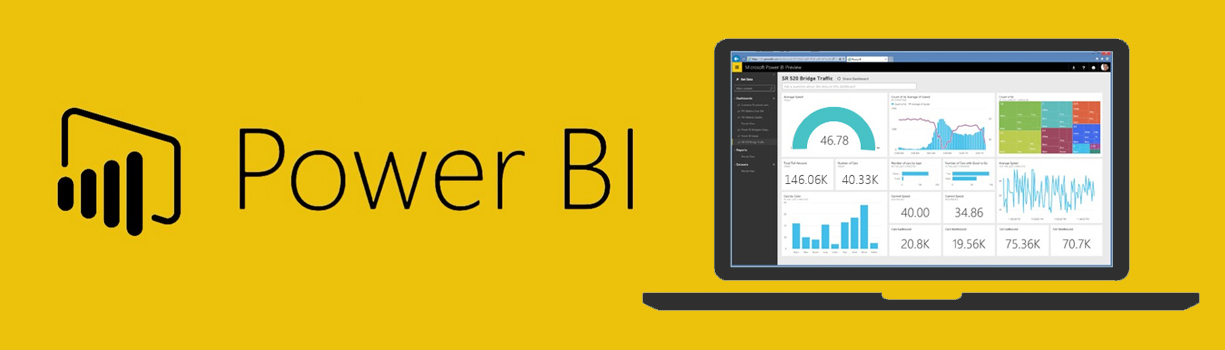
\includegraphics[width=0.8\textwidth]{Images/powerBI.png}
    \end{center}
\end{figure}

Key Features:
\begin{itemize}
    \item \textbf{Data Connectors:} Integrates with a wide range of data
    sources, including databases, cloud services, and real-time data.
    \item \textbf{DirectQuery:} Allows real-time access to large datasets
    without importing data into Power BI, improving performance and scalability.
    \item \textbf{Customizable Dashboards:} Users can create personalized
    dashboards to monitor key metrics like flight delays.
    \item \textbf{Real-time Data Streaming:} Capabilities to visualize real-time
    data for up-to-date decision-making.
    \item \textbf{Advanced Analytics:} Supports machine learning models, DAX
    (Data Analysis Expressions), and custom calculations for deeper insights.
    \item \textbf{Interactive Visualizations:} Offers a variety of
    visualizations like bar charts, line graphs, and heatmaps to represent
    trends and data patterns.
\end{itemize}

Power BI’s DirectQuery feature is especially beneficial for big data analysis,
allowing real-time access to large and continuously changing datasets. This
capability, combined with Power BI’s other features like customizable dashboards
and advanced analytics, makes it an excellent choice for visualizing and
analyzing flight delay data in this project.
\section{How the application works}
\subsection{Workflow}
The aviation data application operates through a structured workflow that
involves \textbf{Data Collection, Data Storage and Processing, and Analytics and
Reporting}. This approach ensures that vast amounts of real-time data are
collected, efficiently processed, and converted into actionable insights.

\subsection*{Step 1: Data collection}
The application’s workflow begins with \textbf{Data Collection}, where
information is gathered from multiple aviation-related sources such as
FlightAware, Flightradar24, Airline On-Time Statistics, and Flight Air Map.
These sources provide essential data, including flight schedules, delays, and
real-time positioning of aircraft. To create a comprehensive view of operations,
the application integrates this data in real-time from additional sources like
air traffic control systems and weather services, which helps in forming a
complete picture of flight conditions necessary for informed decision-making.

\subsection*{Step 2: Data storage and processing}
Once collected, data is organized and processed in the \textbf{Data Storage and
Processing} stage. Initially, raw data from diverse sources is stored in a data
lake (blob storage), which can accommodate various unstructured data types. To
enable real-time data transformation, the application employs PySpark, allowing
for the rapid processing of large datasets. The processed data is then stored in
a Yugabyte data warehouse, optimized for complex querying and analysis,
providing an efficient setup for generating analytical insights. This data is
structured using a star schema, a modeling technique that organizes information
into fact and dimension tables, which facilitates efficient retrieval and
supports detailed analysis.

\subsection*{Step 3: Analytics and reporting}
In the \textbf{Analytics and Reporting} stage, the application analyzes
historical and real-time flight data to identify potential flight delays. This
data-driven approach enables the aviation industry to shift from reactive to
proactive operations, allowing better anticipation of delays. Additionally, the
application visualizes key performance indicators (KPIs) and other relevant
metrics related to delays through user-friendly dashboards. These visualizations
make complex data accessible and interpretable, supporting quick, data-driven
decision-making and improving overall operational efficiency.

\subsection{Dataflow}

\begin{figure}[h]
\centering
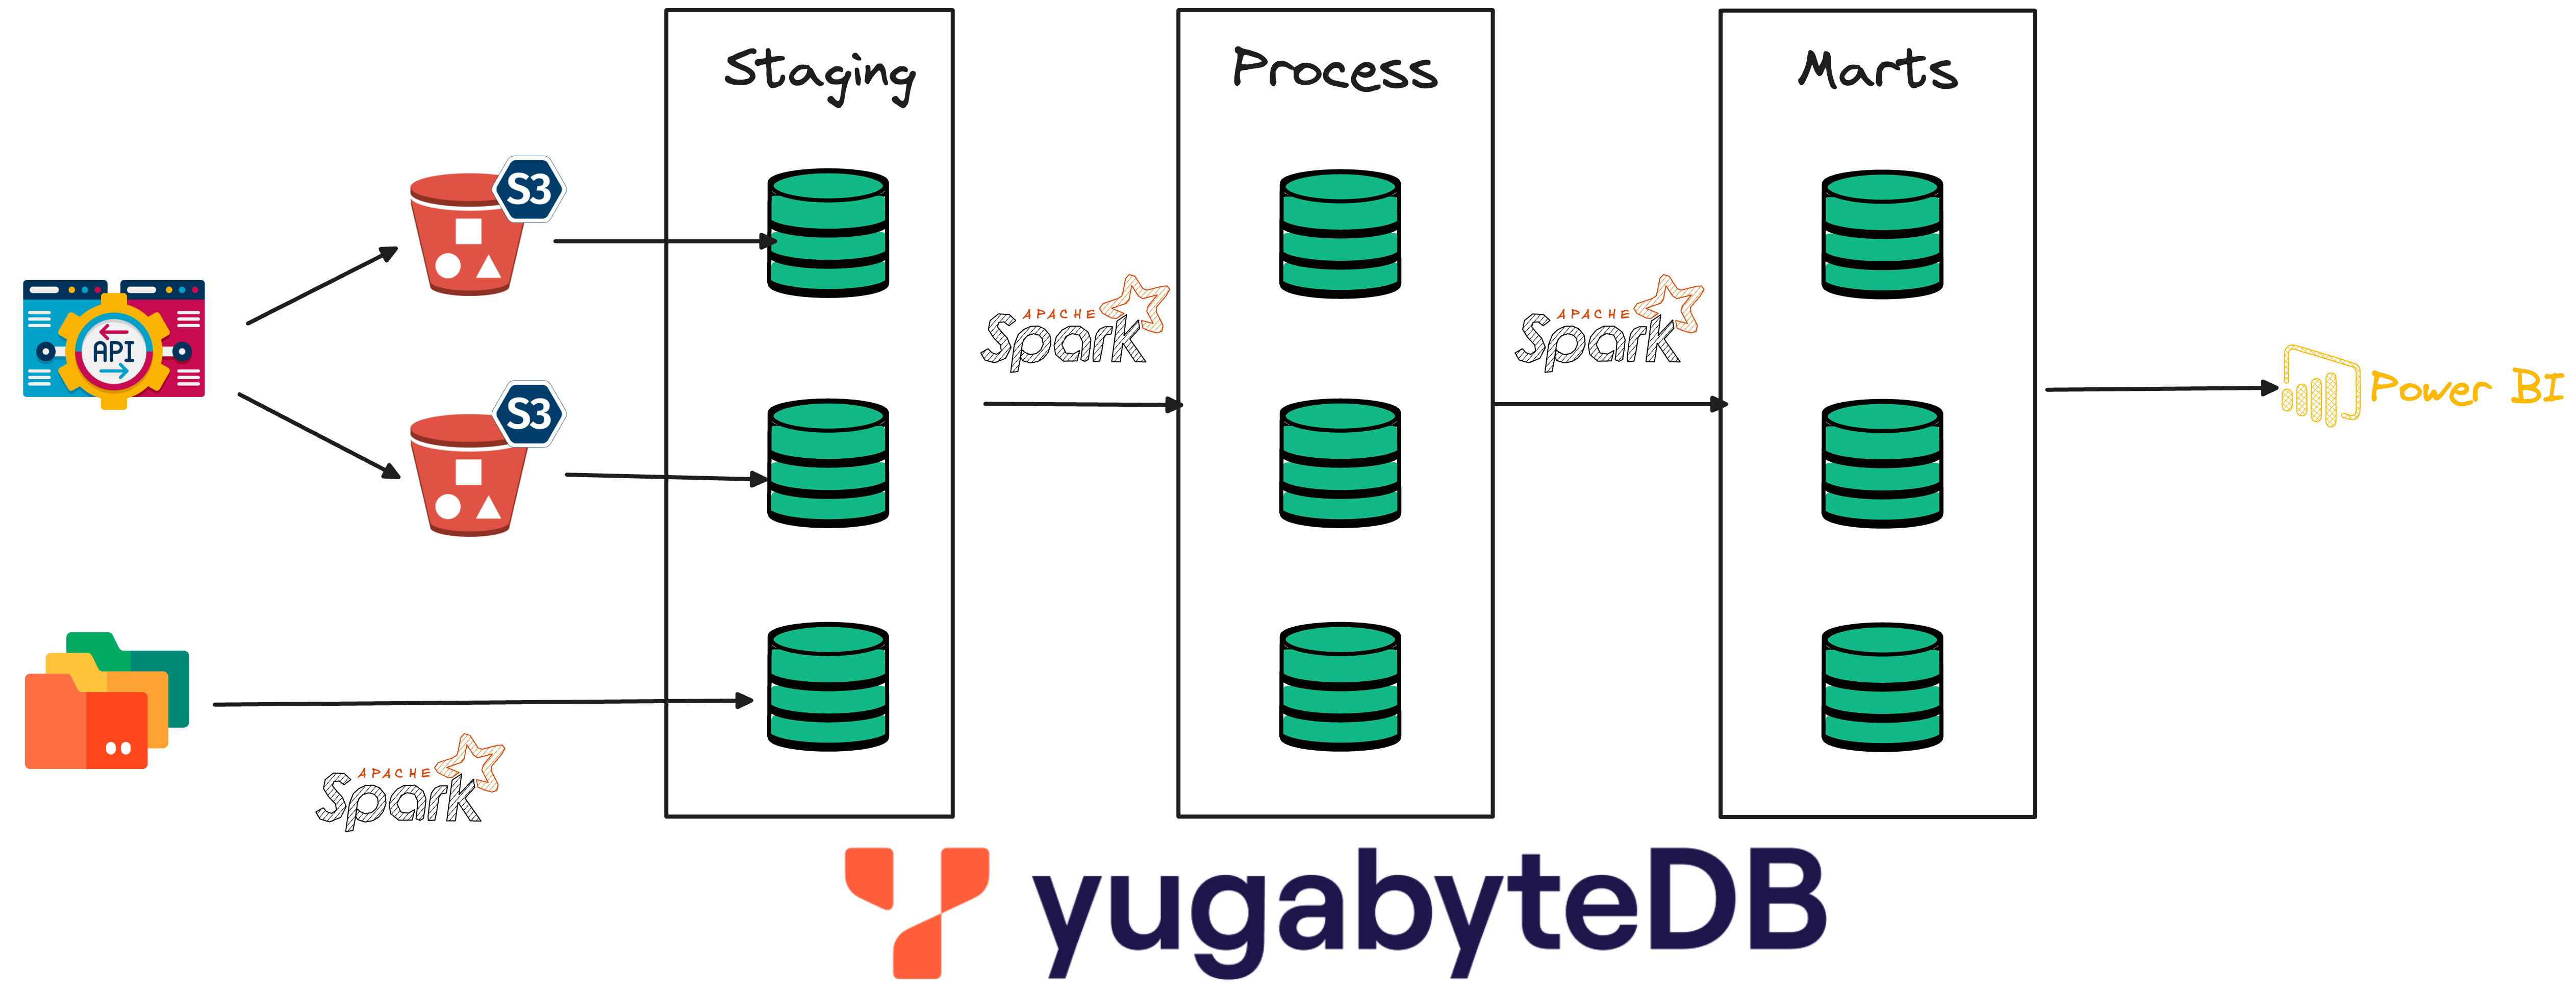
\includegraphics[width=\textwidth]{Images/dataflow.png}
\vspace{1em}
\caption{Dataflow architecture showing the stages of data ingestion, processing, and analytics}
\label{fig:dataflow}
\end{figure}

The dataflow depicted in Figure \ref{fig:dataflow} demonstrates a modern data
engineering pipeline leveraging scalable cloud and big data technologies. The
flow comprises three distinct stages. In the data ingestion stage, data is
sourced from APIs and file systems. APIs write data directly into S3 buckets,
which serve as a staging layer, while files from folders are also uploaded into
S3 for processing.

In the staging layer, the ingested data is stored in S3 buckets to serve as a
transient layer before processing. From S3, data is migrated to YugabyteDB, a
distributed SQL database, for temporary structured storage. The processing layer
involves Apache Spark, which processes data from the staging layer, applying
transformation, cleaning, and business logic to the data. The processed data is
then saved back to YugabyteDB, where it is structured for downstream analytics.

Finally, in the data marts layer, the cleaned and transformed data is further
organized into data marts, making it available for consumption through
analytical tools. Power BI is used to create dashboards and visualizations from
the data stored in these data marts.

\subsection{Deployments}

\begin{figure}[h]
\centering
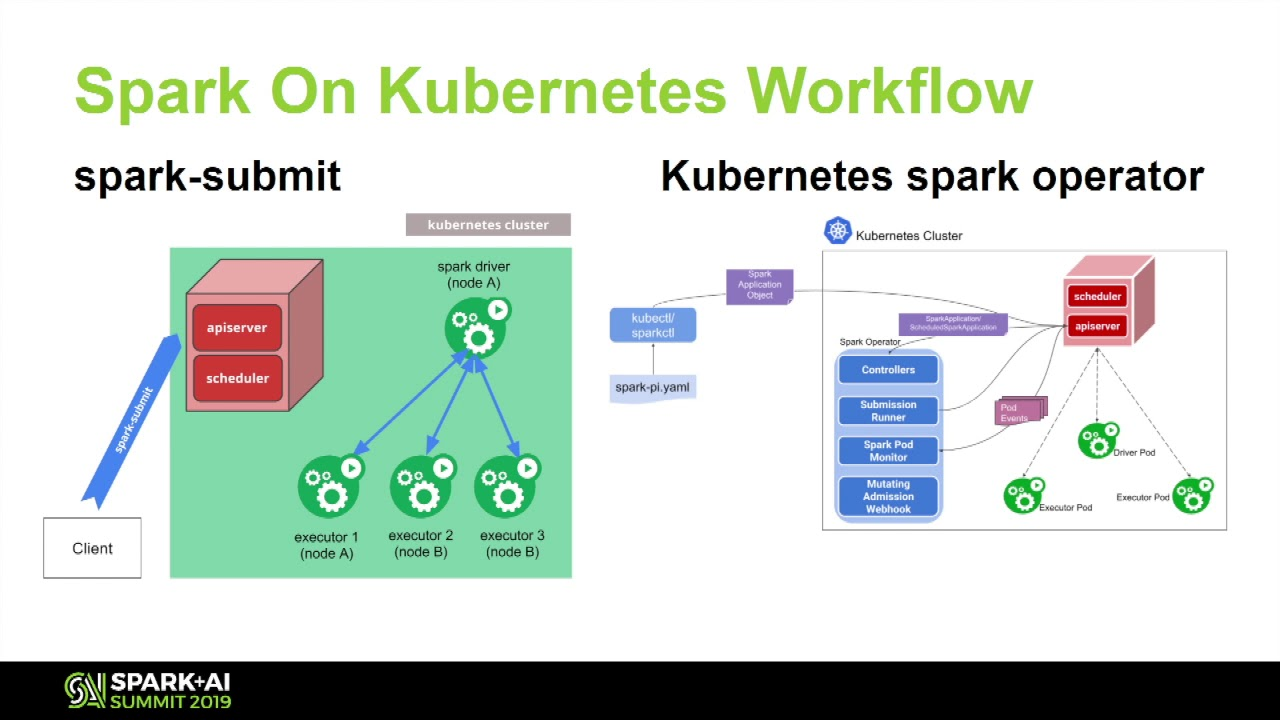
\includegraphics[width=\textwidth]{Images/sparkdevops.png}
\vspace{1em}
\caption{Spark deployment on Kubernetes using AKS, illustrating the use of
\texttt{spark-submit} and the Kubernetes Spark Operator
\cite{spark_ai_summit_2019}}
\label{fig:sparkdevops}
\end{figure}

The deployment depicted in Figure \ref{fig:sparkdevops} shows how Apache Spark
can be integrated with Kubernetes clusters using Azure Kubernetes Service (AKS).
There are two different approaches for deploying Spark on Kubernetes,
represented in the diagram. The first approach is using spark-submit, which
allows the submission of Spark jobs using the \texttt{spark-submit} command to
the Kubernetes cluster. The Kubernetes cluster has an API server and a scheduler
that manage the allocation of nodes for executing the Spark driver and
executors.

The second approach is through the Kubernetes Spark Operator, which simplifies
the management of Spark applications. A \texttt{SparkApplication} object defines
the application, which is managed by the Spark Operator on the cluster. The
Spark Operator handles the submission, monitoring, and scaling of Spark jobs,
automating much of the workflow. This deployment strategy helps efficiently
manage resources, ensuring scalability and reliability of data processing.

\subsection{Benefits to stakeholders}
The aviation data application provides significant benefits to various
stakeholder groups, each of which plays a crucial role in ensuring smooth and
efficient operations:

\begin{itemize}
    \item \textbf{Operational Teams:} With access to real-time insights,
    operational teams can improve scheduling and resource allocation. This
    capability allows for better alignment of flights, staff, and equipment,
    leading to enhanced efficiency and minimizing potential disruptions.
    \item \textbf{Maintenance Crews:} Management teams benefit from data-driven
    strategic planning based on both historical and real-time flight operation
    data. This comprehensive insight allows managers to make informed decisions,
    optimize resource allocation, and plan for the future, ultimately driving
    organizational success and resilience.
    \item \textbf{Management:} Management teams benefit from data-driven
    strategic planning based on both historical and real-time flight operation
    data. This comprehensive insight allows managers to make informed decisions,
    optimize resource allocation, and plan for the future, ultimately driving
    organizational success and resilience.
    \item \textbf{Passengers:} Passengers experience an enhanced travel
    experience due to fewer delays, optimized scheduling, and reduced
    cancellations. By improving operational efficiency and reliability, the
    application contributes to a smoother journey for travelers, increasing
    customer satisfaction and building loyalty.
\end{itemize}
$\quad$Overall, the application’s capabilities in real-time data processing,
predictive maintenance, and strategic planning empower each stakeholder group,
fostering a more efficient, proactive, and customer-centric aviation industry.

\section{Implementation plan}
The implementation plan for the aviation data application is divided into four
phases: \textbf{Planning and Requirements Gathering, Development, Testing, and
Deployment}. Each phase is designed to ensure that the application is built,
tested, and deployed effectively, meeting both technical and business
objectives.

\subsection*{Phase 1: Planning and Requirements Gathering}
This initial phase, lasting 1.5 weeks (Week 3 to mid-Week 4), involves defining
the project scope and objectives. It includes identifying the necessary data
sources, such as FlightAware, Flightradar24, and Flight Air Map, and outlining
infrastructure requirements. This foundational phase sets the direction for the
subsequent development work.

\subsection*{Phase 2: Development}
Spanning 2.5 weeks (mid-Week 4 to Week 7), this phase focuses on setting up the
big data infrastructure. This involves configuring Yugabyte for data
warehousing, establishing blob storage for the data lake, and utilizing PySpark
for distributed data processing. Additionally, data ingestion and processing
pipelines are developed to handle real-time data from various sources, ensuring
the system is equipped for efficient data handling.
\subsection*{Phase 3: Testing}
Lasting 2 weeks (Week 7 to Week 9), this phase includes pilot testing with
selected flight routes to validate data accuracy and system performance. Stress
testing is also conducted to ensure that the application can scale effectively
under heavy data loads, confirming its robustness before full deployment.
\subsection*{Phase 4: Deployment}
The final phase, taking 2 weeks (Week 9 to Week 11), involves the full-scale
implementation of the system, making it fully operational. This deployment phase
ensures that the application is accessible to stakeholders, with all
functionalities optimized for real-world use.

\section{Result}
Our group has developed an application designed to streamline the collection,
processing, and analysis of flight data. The application collects data from
multiple trusted sources, ensuring the accuracy and reliability of the
information. These raw datasets are then stored in a Data Lake, which serves as
a centralized repository for efficient and scalable storage, allowing future use
and exploration.\\
To process the stored data, we utilized PySpark, a powerful tool for distributed
data processing, ensuring that the data is cleaned, transformed, and prepared
for analysis. After processing, the structured data is stored in Yugabyte, a
distributed SQL database known for its scalability and fault tolerance. This
enables fast, reliable querying and supports advanced analytical operations.\\
For visualization and reporting, our team integrated Power BI to create
customized dashboards. These dashboards are tailored to display critical
insights such as flight delays, operational trends, and carrier performance. By
leveraging the dynamic capabilities of Power BI, users can interact with the
data in real-time, drill down into specific metrics, and generate reports suited
to their requirements.\\
This workflow demonstrates an end-to-end solution for flight data analysis,
incorporating robust data engineering practices and intuitive analytics tools to
deliver actionable insights.\\

Below are some charts and graphs created with powerBI:
\begin{figure}[H]
    \begin{center}
        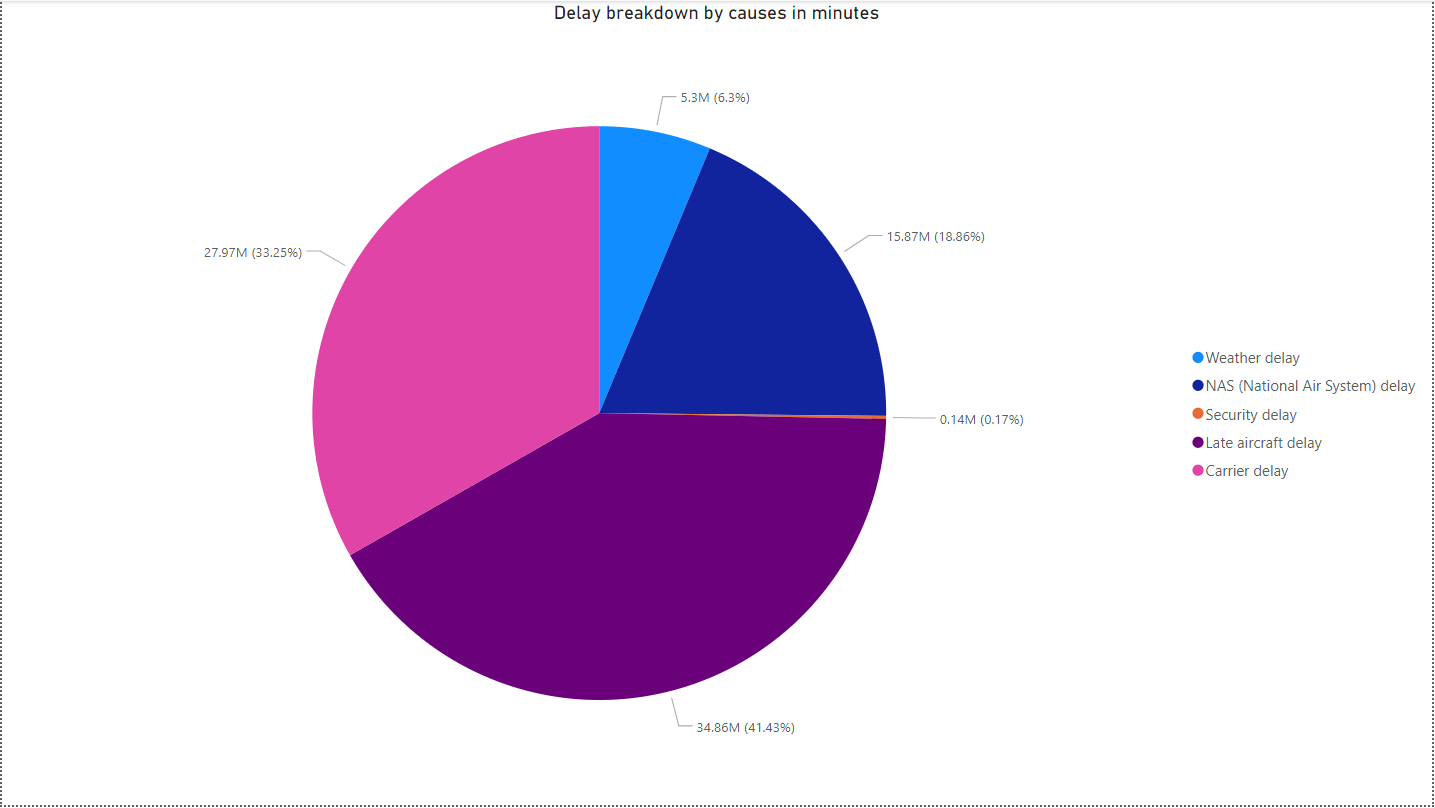
\includegraphics[width=\textwidth]{Images/chart1.png}
        \newline
        \caption{Delay breakdown by causes in minutes}
    \end{center}
\end{figure}
\begin{figure}[H]
    \begin{center}
        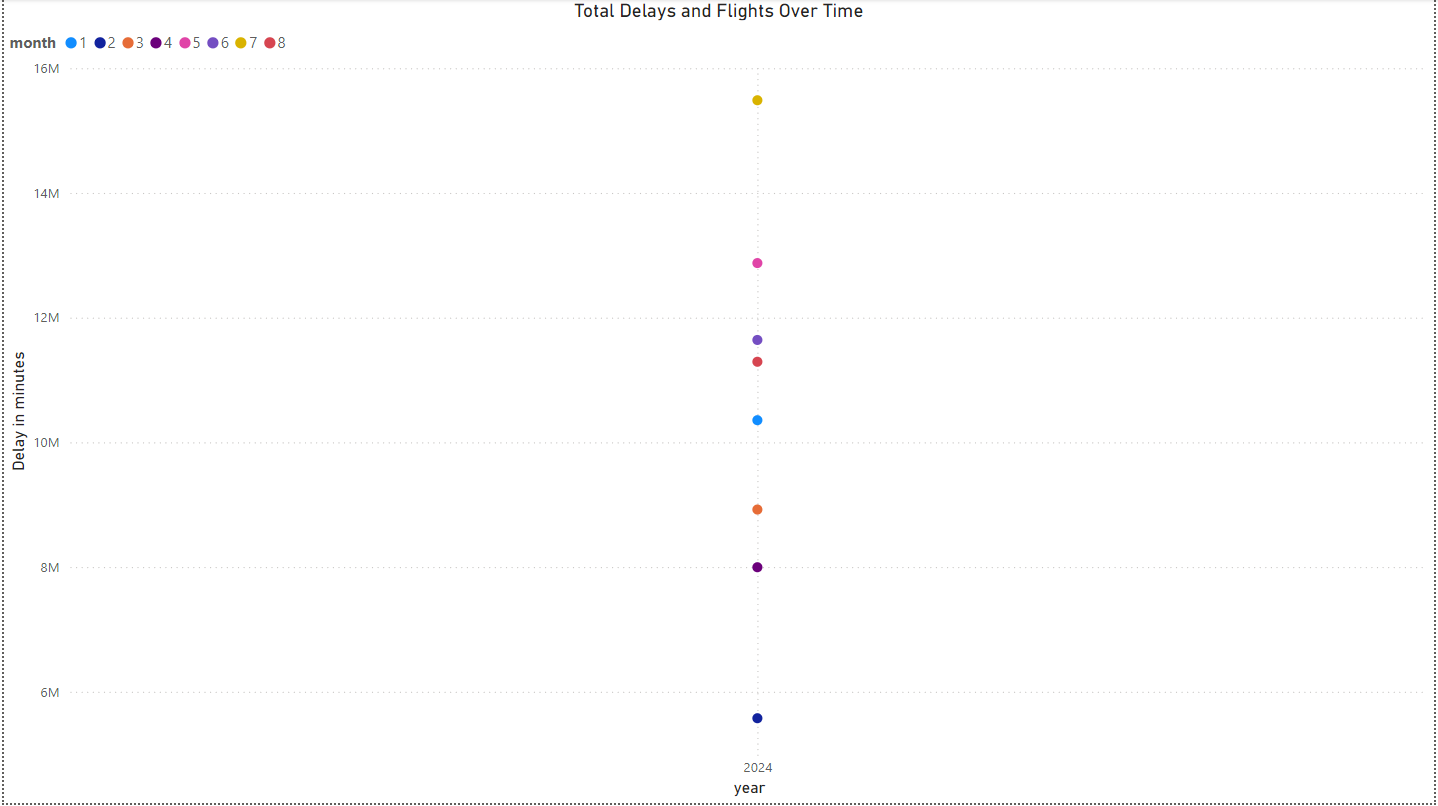
\includegraphics[width=\textwidth]{Images/chart2.png}
        \newline
        \caption{Delay over time}
    \end{center}
\end{figure}
\begin{figure}[H]
    \begin{center}
        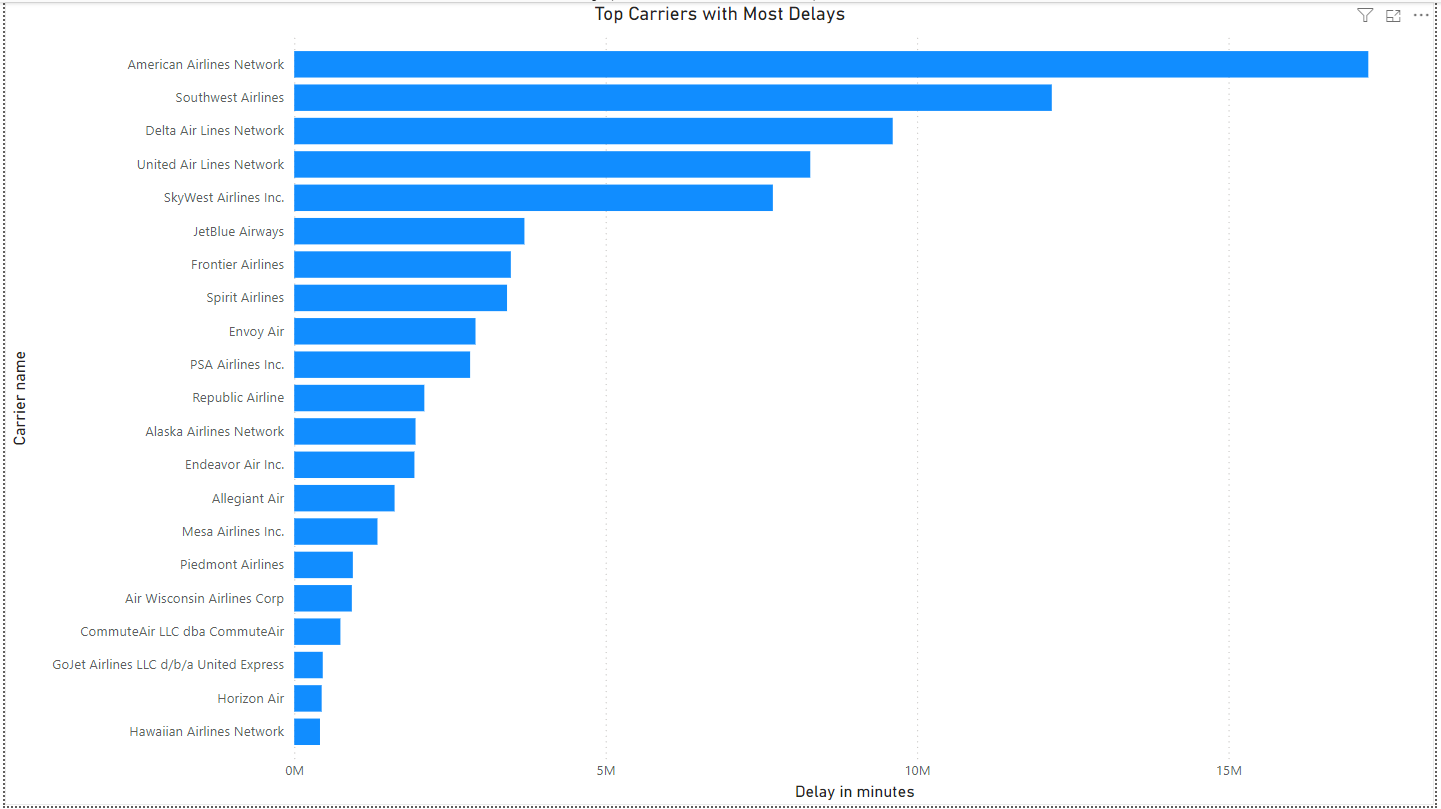
\includegraphics[width=\textwidth]{Images/chart3.png}
        \newline
        \caption{Delay by carrier}
    \end{center}
\end{figure}
\begin{figure}[H]
    \begin{center}
        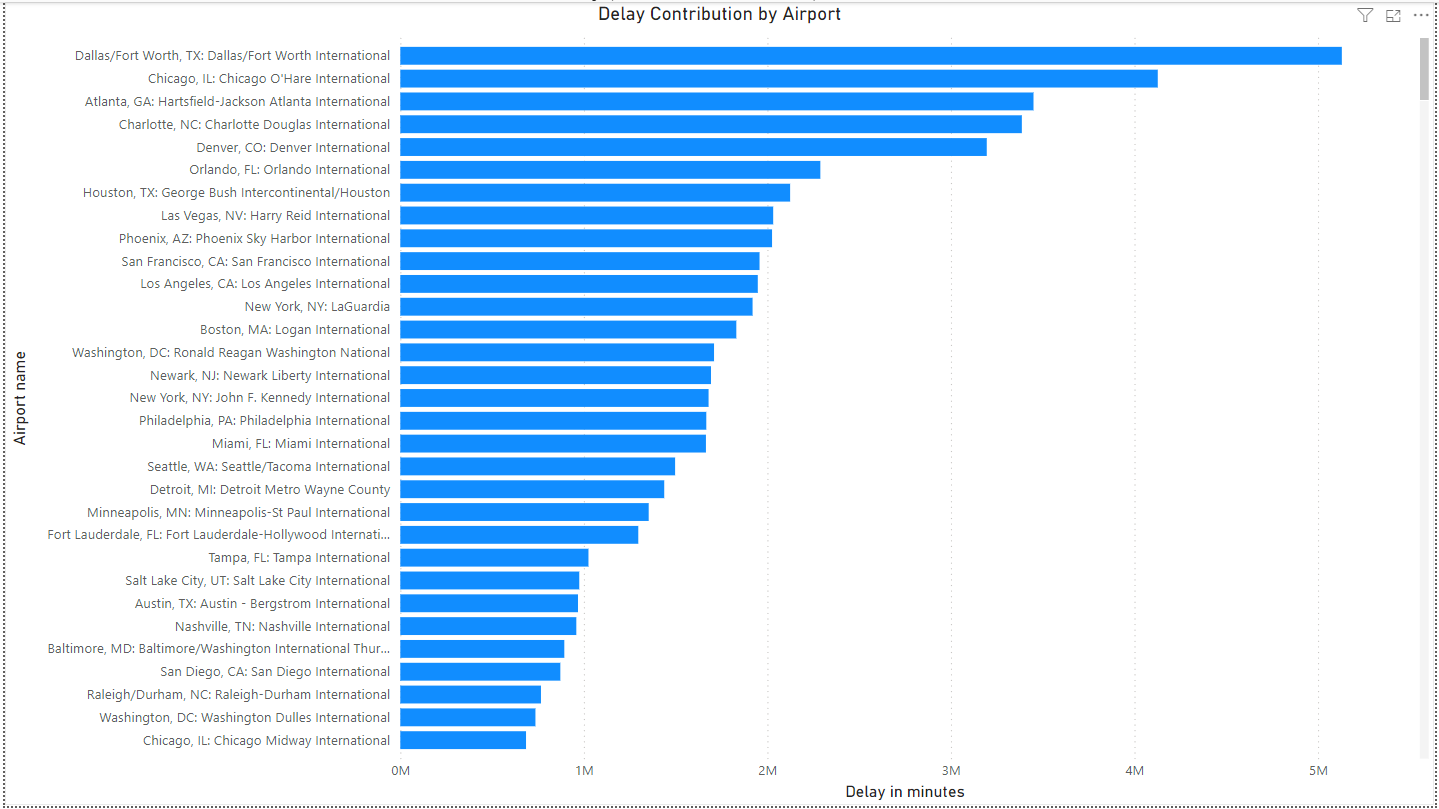
\includegraphics[width=\textwidth]{Images/chart4.png}
        \newline
        \caption{Delay by airport}
    \end{center}
\end{figure}
\begin{figure}[H]
    \begin{center}
        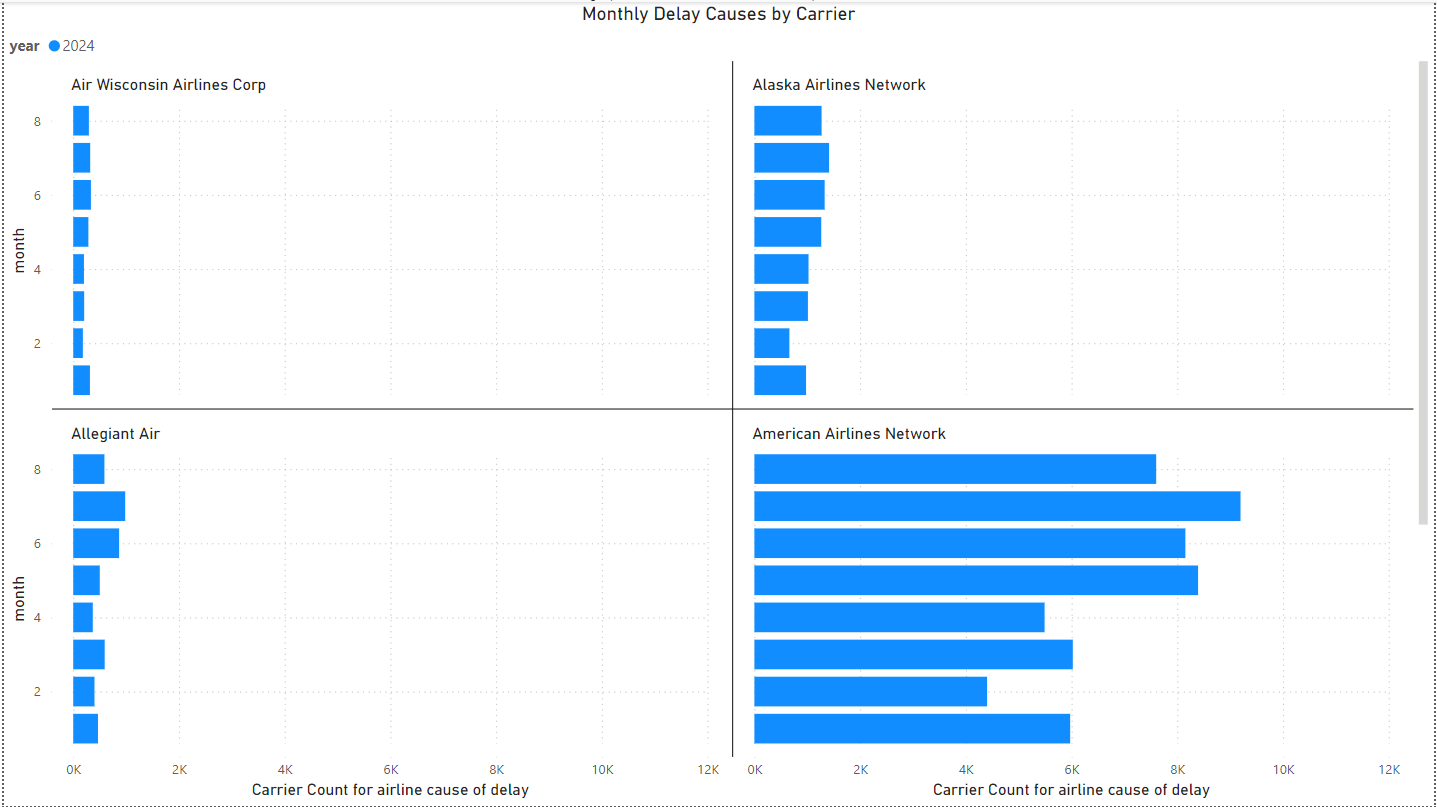
\includegraphics[width=\textwidth]{Images/chart5.png}
        \newline
        \caption{Monthly delay cause by carrier}
    \end{center}
\end{figure}
\begin{figure}[H]
    \begin{center}
        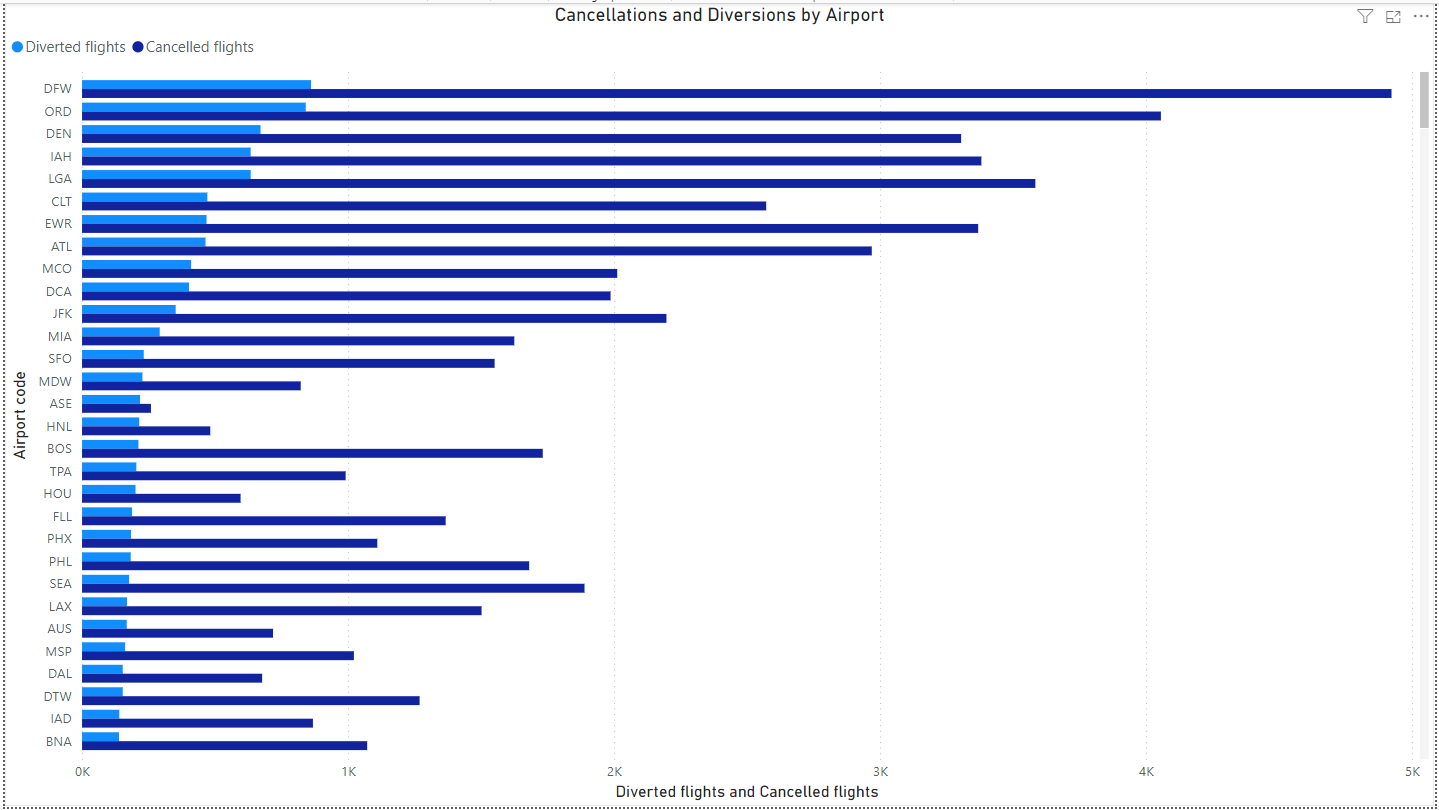
\includegraphics[width=\textwidth]{Images/chart6.png}
        \newline
        \caption{Cancellations and diversions by airport}
    \end{center}
\end{figure}
\begin{figure}[H]
    \begin{center}
        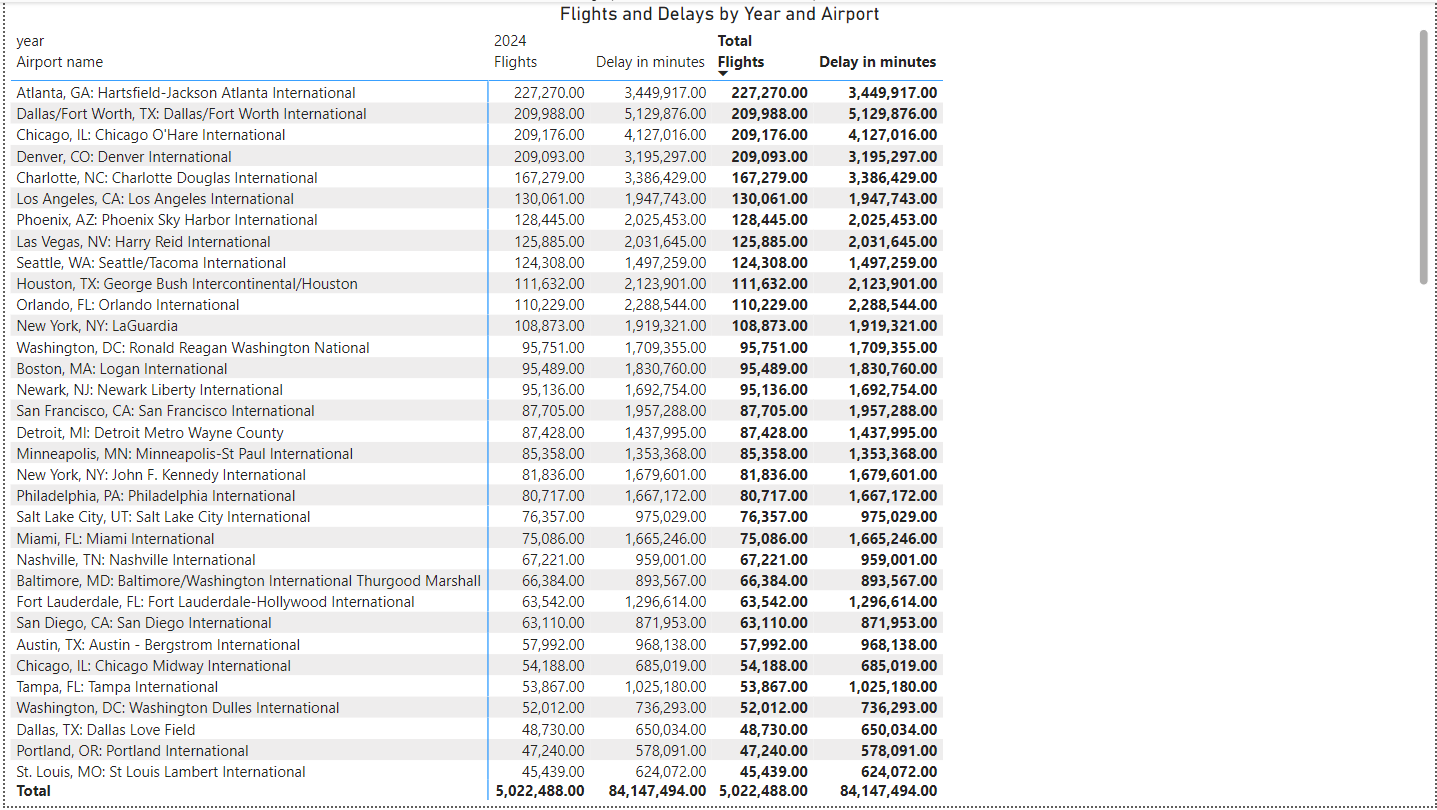
\includegraphics[width=\textwidth]{Images/chart7.png}
        \newline
        \caption{Flights and delay by year and airport}
    \end{center}
\end{figure}
\begin{figure}[H]
    \begin{center}
        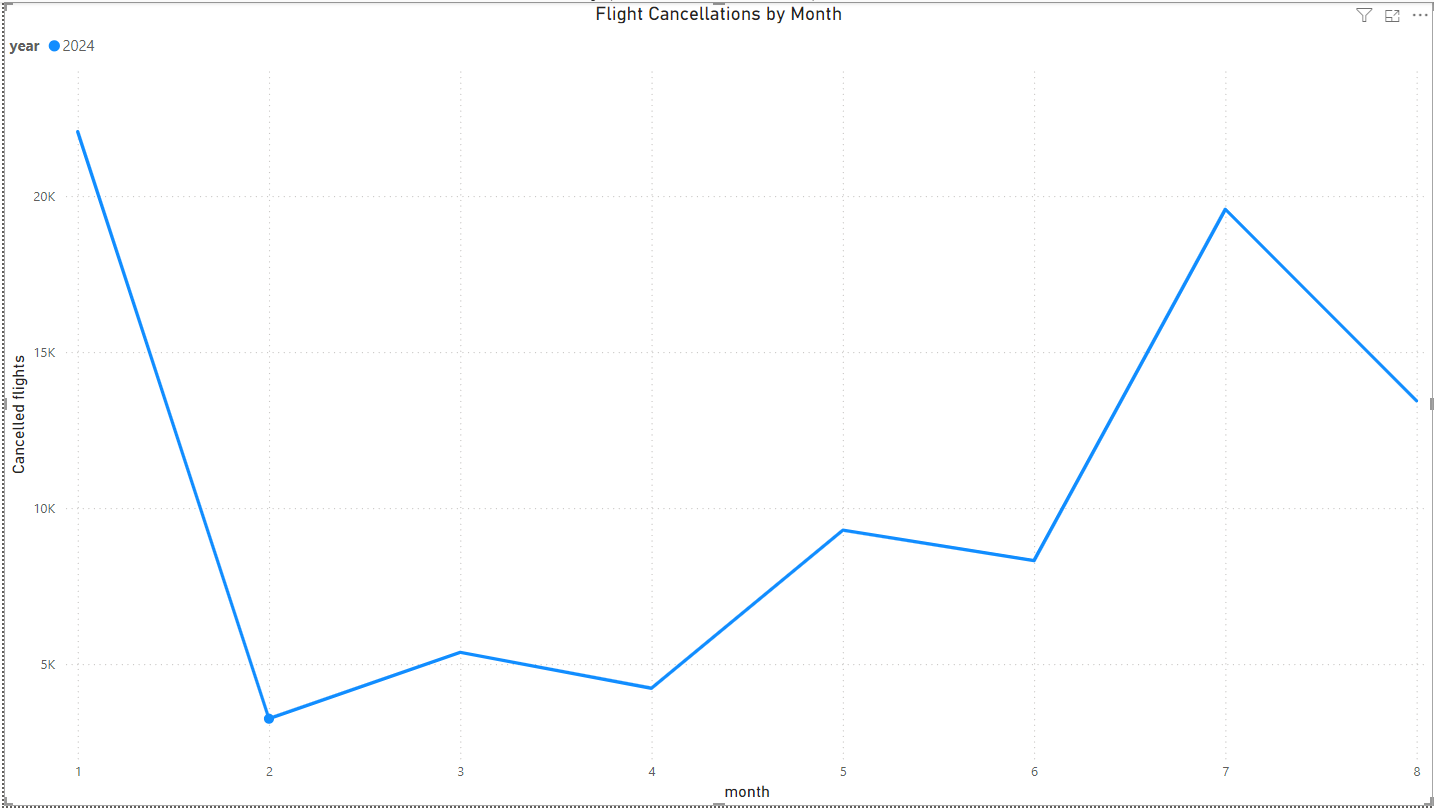
\includegraphics[width=\textwidth]{Images/chart8.png}
        \newline
        \caption{Flight cancellations by month}
    \end{center}
\end{figure}

\section{Evaluation}
\subsection{Data Evaluation}
Data was collected from \textbf{FlightAware, Flightradar24, Flight Air Map, and the FAA}, providing comprehensive aviation information like flight schedules, tracking, and delays.

\textbf{Data Cleaning \& Transformation}\\
The data underwent an \textbf{ETL process:}
\begin{itemize}
    \item \textbf{Cleaning:} Removed duplicates, standardized formats, and resolved missing values.
    \item \textbf{Enrichment:} Merged data from various sources for deeper insights.
    \item \textbf{Loading: } Stored in a Star Schema model in the Data Warehouse.
\end{itemize}

\textbf{Storage and Quality}
\begin{itemize}
    \item Schema: Includes a fact table for flight metrics and dimensions like carrier\_dim, airport\_dim, and time\_dim.
    \item Volume: Handles millions of records.
\end{itemize}

\subsection{System Evaluation}
\textbf{Scalability}\\
The system was designed to handle increasing data volumes efficiently:
\begin{itemize}
    \item \textbf{MinIO:} Provides scalable and fault-tolerant storage as a Data Lake.
    \item \textbf{PySpark:} Supports distributed data processing for large datasets.
    \item \textbf{YugabyteDB:} Ensures high-performance querying and scalability as a distributed Data Warehouse.
\end{itemize}

\textbf{Performance}
\begin{itemize}
    \item \textbf{ETL to Visualization Workflow:} The pipeline ensures processed data is quickly available for PowerBI dashboards.
    \item \textbf{Query Execution:} YugabyteDB enabled fast analytical queries on the Star Schema.
\end{itemize}

\textbf{Fault Tolerance}
\begin{itemize}
    \item \textbf{MinIO:} Ensures data redundancy and recovery in case of failures.
    \item \textbf{YugabyteDB:} Maintains high availability with distributed architecture.
\end{itemize}

\textbf{Integration}\\
The technologies integrate seamlessly:
\begin{itemize}
    \item MinIO serves as the raw data repository for PySpark processing.
    \item PySpark outputs are loaded into YugabyteDB, supporting downstream analytics.
    \item PowerBI connects to YugabyteDB for visualization, providing real-time insights.
\end{itemize}

\textbf{Cost Efficiency}\\
Utilized open-source technologies to minimize infrastructure costs while ensuring robust performance.

\textbf{Visualization Capabilities}
\begin{itemize}
    \item \textbf{Interactive Dashboards:} Visualizations include flight delays, airport traffic, and carrier performance with filters for time, location, and other dimensions.
    \item \textbf{Real-Time Insights:} Automated data refresh cycles keep dashboards up-to-date.
\end{itemize}

\nocite{*}
\bibliographystyle{plainnat}

\bibliography{refs}

\end{document}